\chapter{Replication And Synchronization}
Replication refers to the concept of storing several copies of a data record at different database servers. These \textit{copies} are called \textbf{replicas} and the \textit{number of copies} is called the \textbf{replication factor}. 
When applying replication to large data sets:
\begin{itemize}
    \item First a fragmentation of the data set is obtained
    \item Fragments are replicated among a distributed database system
    \item Replication improves reliability and availability of a distributed system because replicas can serve as backup copies whenever one of the servers fails and becomes unavailable
    \item It enables load balancing or data locality
    \item This kind of concurrent accesses to different replicas lead to consistency problems
\end{itemize}

\section{Replication Models}
Replication has several \textbf{advantages:}
\begin{itemize}
    \item It improves the \textbf{reliability} by offering higher data availability
    \item It offers \textbf{lower latency} by enabling load balancing, data locality and parallelization
\end{itemize}
These two advantages implies respectively two a major \textbf{disadvantages}:
\begin{itemize}
    \item \textbf{Consistency problems}: because when a user updates a data record at one server, network delays or even network failures may prevent the database system from updating all other replicas of the data record quickly
    \item \textbf{Concurrency problem:} where two or more users might concurrently update the same data record on different replicas
\end{itemize}

\begin{tcolorbox}
The two basic models of replication are \textbf{master-slave} and \textbf{multi-master} replication. While the \textit{consistency problem} exists for both, the \textit{concurrency problem} is \textbf{avoided} in the \textbf{master-slave} case but at the cost of higher latency for write requests
\end{tcolorbox}

\subsection{Master-Slave Replication}
\begin{itemize}
    \item In master-slave replication, \textit{write} requests are handled only by a \textit{single server} that is called the \textbf{master}.
    \item After a write, the master is responsible for \textit{updating} all other servers that hold a replica, called \textbf{slaves}
    \item Read requests can be accepted by both the master and the slaves
\end{itemize}
\begin{figure}[!h]
        \centering
        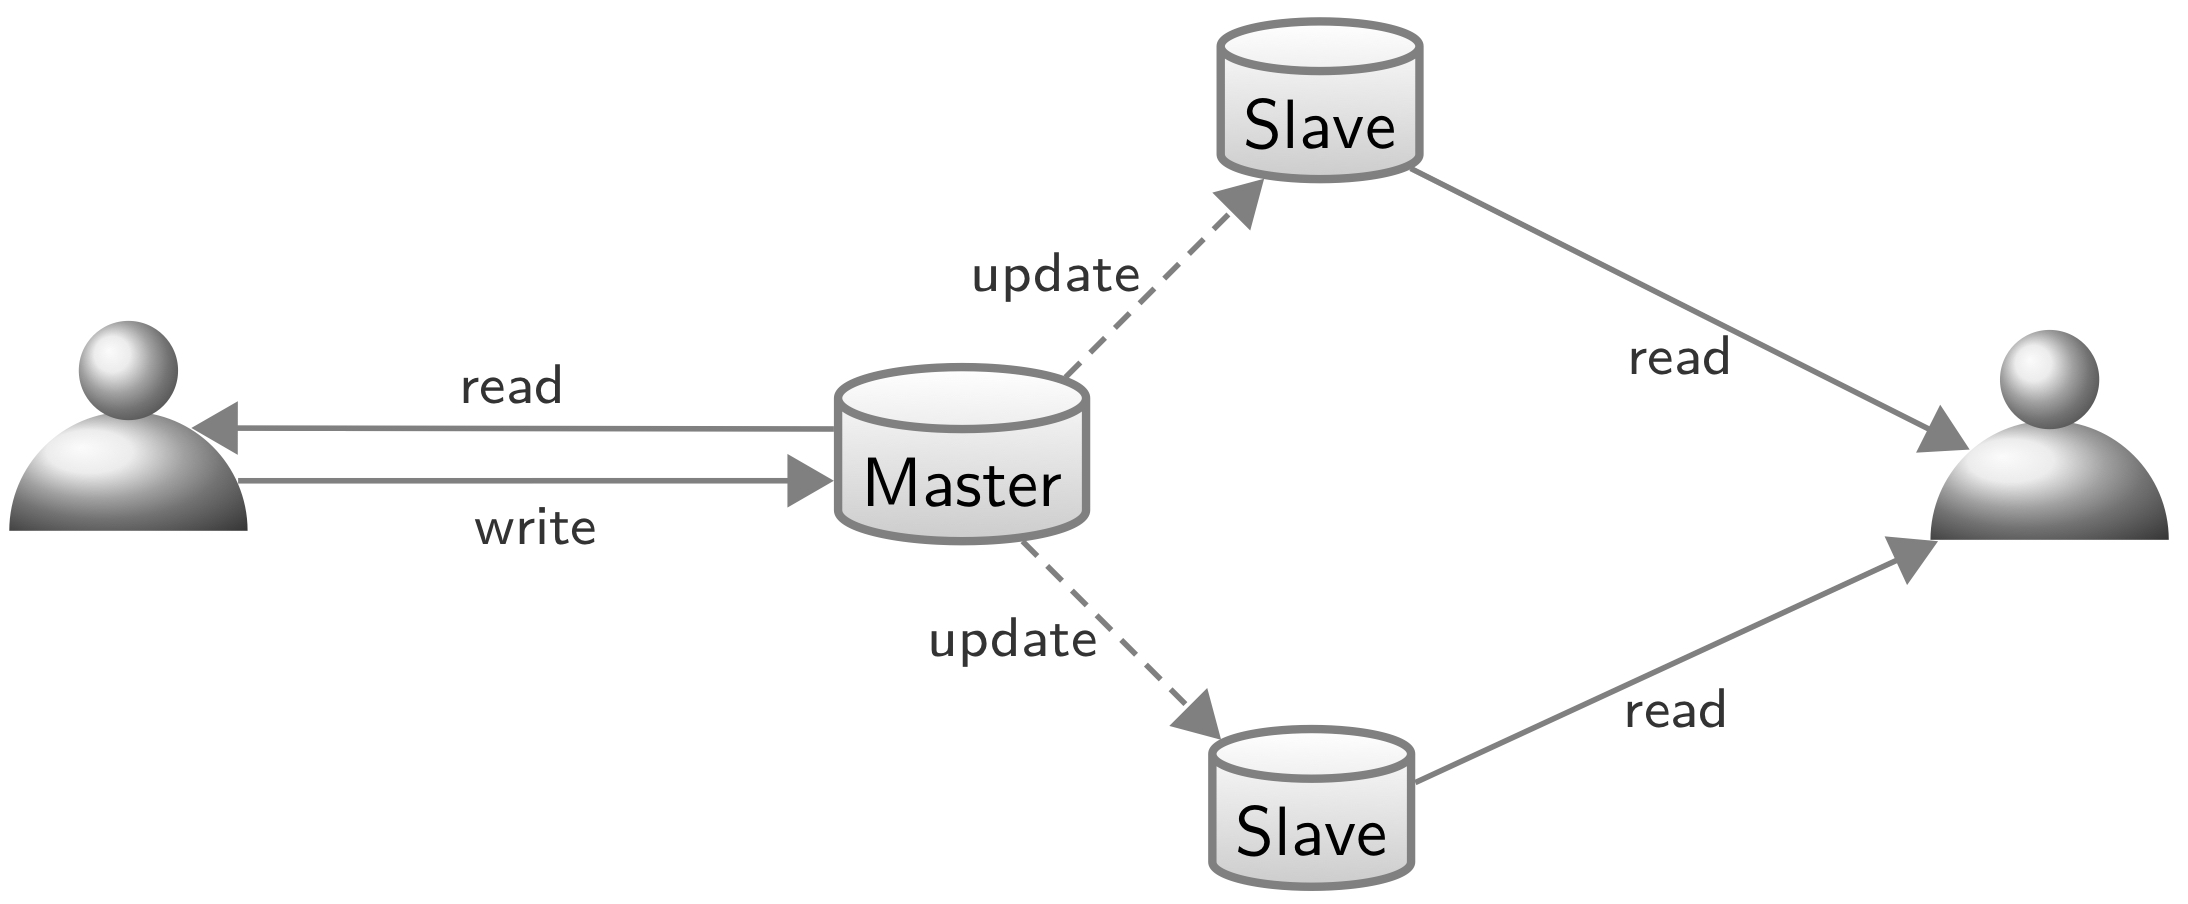
\includegraphics[width=0.8\linewidth]{images/AdvancedDataManagment/replication_and_synchronization/master_slave_replication.jpeg}
        \caption{A Master-slave replication}
    \end{figure}

Master-slave replication offers enough \textbf{redundancy} in case of a \textbf{master failure}: when the master fails, \textit{one of the slaves} can be \textbf{elected} to be the \textbf{new master} and all write request are redirected to it.

Having a \textit{single master server} for all write requests in the database system is a \textbf{bottleneck} that slows down the processing of writes tremendously.
\begin{itemize}
    \item A solution is to \textit{partition} the set of all data records into \textbf{disjoint subsets} and to each such \textit{subset} assign \textit{one server} as the \textbf{master server}
    \item In combination with data partitioning, data records in the same partition are copied to the same replication servers and one of the servers is designated master for the entire partition while the others act as slaves
\end{itemize}
\begin{figure}[!h]
        \centering
        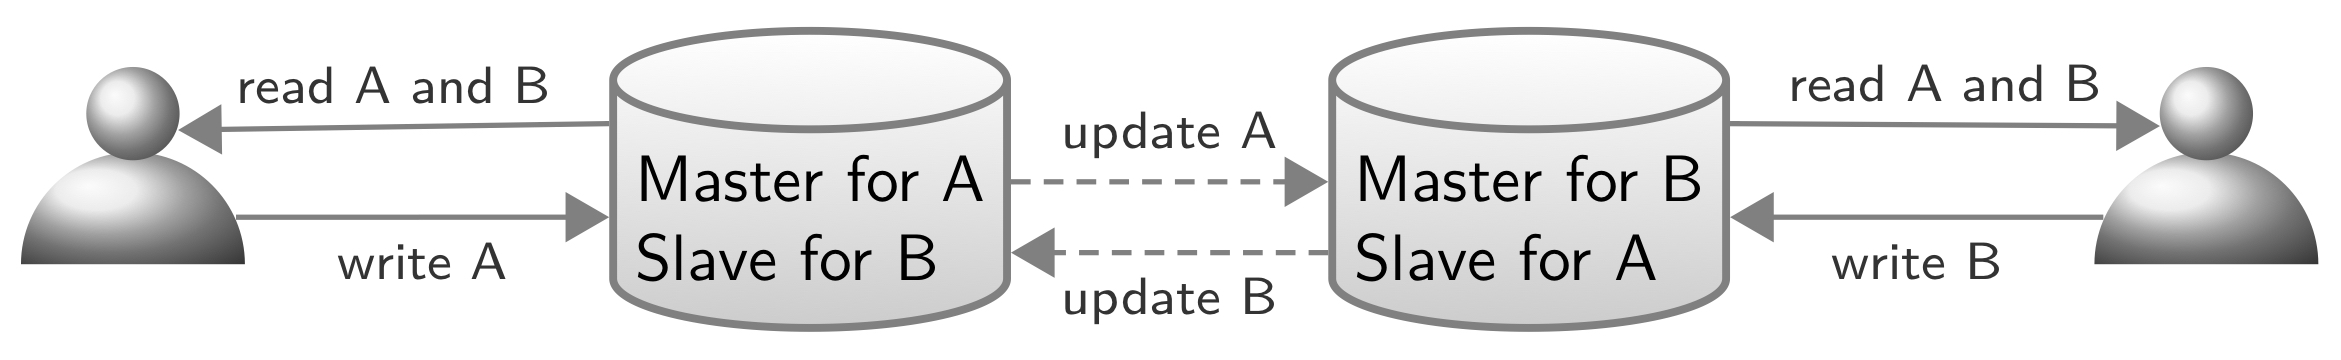
\includegraphics[width=0.8\linewidth]{images/AdvancedDataManagment/replication_and_synchronization/ms_rep_mul_records.jpeg}
        \caption{Master-slave replication with multiple records}
    \end{figure}


\subsection{Multi-Master Replication}
\begin{itemize}
    \item When all servers holding a replica of a data record can process write request, they all act as masters for the data record, this is the case of \textbf{multi-master replication} or \textbf{peer-to-peer replication} (based on the fact that the masters are peers with identical capabilities and they have to synchronize one with the other)
    \item Higher write availability than master-slave replication, because clients can contact any replica server with a write request, parallel requests
    %IMAGE
    \item All servers accept write and read requests for a data item
    \item The servers have to regularly synchronize their state among themselves
    \item Due to the \textbf{consistency problem:}
    \begin{itemize}
        \item Clients may retrieve \textit{outdated data} whenever the replica answering the client’s read request has \textit{not finished the synchronization process}
    \end{itemize}
    \item Due to the \textbf{concurrency problem:}
    \begin{itemize}
        \item Replicas may be in conflict when different clients wrote to different replicas without a synchronization
    \end{itemize}
\end{itemize}
\begin{figure}[!h]
        \centering
        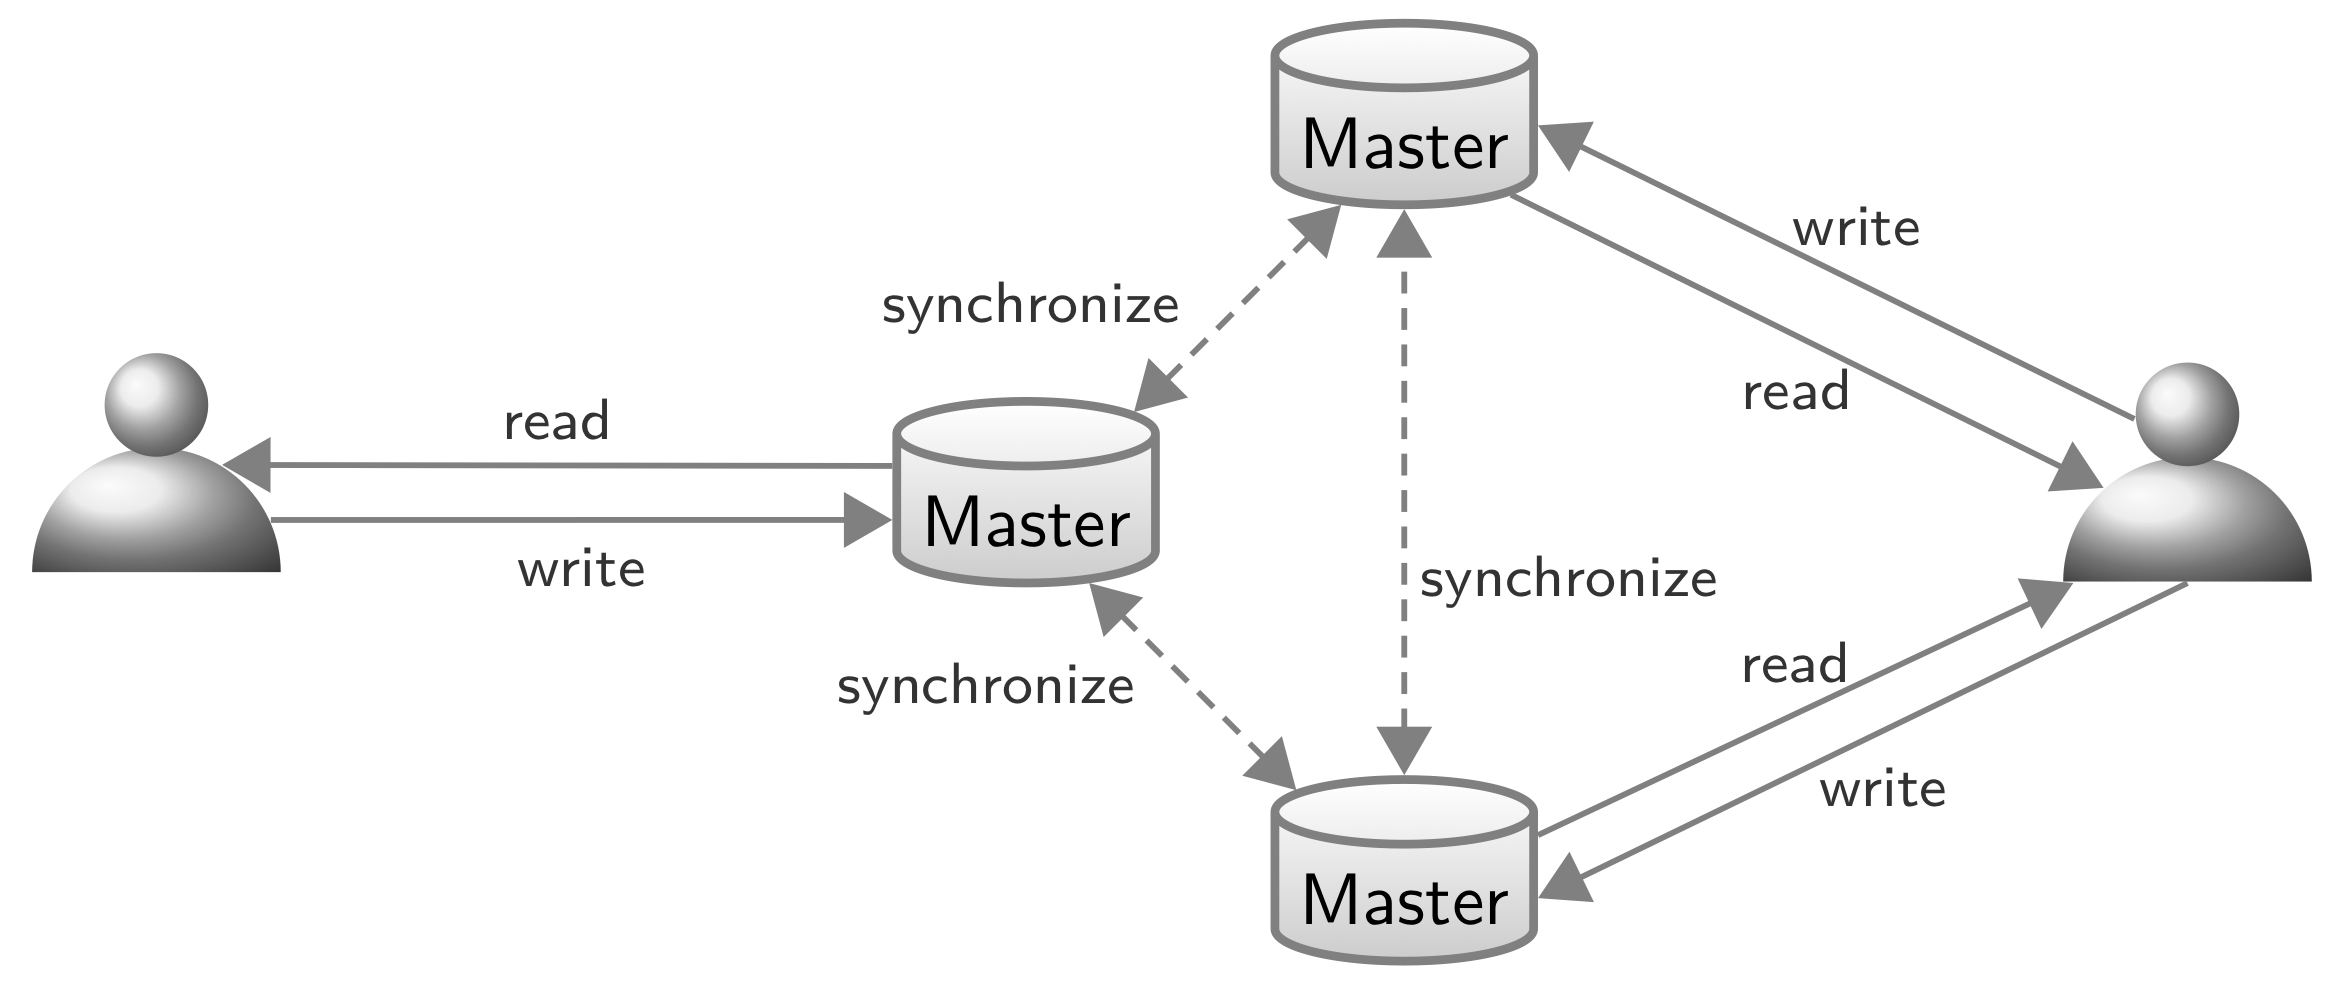
\includegraphics[width=0.8\linewidth]{images/AdvancedDataManagment/replication_and_synchronization/multi_master_replication.jpeg}
        \caption{Multi-master replication}
    \end{figure}